\chapter{Realization} \label{chapter:realization}
After having discussed the basic concept of the approach in the previous chapter, in this chapter, an exemplary realization is presented. Previously, three key challenges were identified:
\begin{inparaenum}[(i)]
  \item \emph{reliable, anonymous information exchange},
  \item \emph{isolation}, and
  \item \emph{connectivity} (\cf \ref{sec:challenges}).
\end{inparaenum}
To tackle these challenges, three technologies are proposed:

\begin{enumerate}[(i)]
\item \textbf{DDS} to enable \emph{reliable, anonymous information exchange},
\item \textbf{\docker} as containerization tool to achieve \emph{isolation} and portability of services, and
\item \textbf{\wnet} as means to provide \emph{connectivity} between the containerized services.
\end{enumerate}

In the following, these three tools are presented and it is described how they are leveraged to realize the proof of concept implementation.


\section{Data Distribution Service for Data Exchange}
Data Distribution Service (DDS) is a messaging middleware standard \cite{dds-1.4-standard} for distributed applications governed by the Object Management Group (OMG).\footnote{\url{www.omg.org}} DDS is designed for mission- and business critical systems with real-time requirements. As such, it aims to function in a resource efficient, predictable and reliable manner, and is subject to minimal computational and transport overhead.
Thus, DDS is a great fit for the automotive use case. 

\subsection{Data-Centric Publish-Subscribe}
DDS is fundamentally based on the data-centric publish-subscribe (DCPS) communication paradigm. In the publish-subscribe-style communication, data flows between two kinds of entities: publishers and subscribers. Publishers provide data, while subscribers consume that data. A crucial characteristic of publish-subscribe is that data exchange between the peers is anonymous, \ie , publishers have no way of sending data to individual subscribers. Instead, both communicate by means of a shared, logical medium that takes data samples and forwards them to the appropriate receivers. In the context of DDS, this medium is called \emph{topic}. When subscribers receive a data sample they do not know where that sample originated. Similarly, publishers have no knowledge about where the sent data will end up at---or even if there are any receivers at all. Entities in this system find each other not by way of addressing, but rather on the basis of a shared understanding of what \emph{kind of data} they want to exchange. This approach is called \emph{data centricity}. Data centricity is in contrast to \emph{message centricity}, in which data exchange is driven by \emph{messages}, or \emph{instructions}, which are directed at individual receivers. A prominent example of a message-centric technology is Remote Procedure Call (RPC). To illustrate the difference between the two paradigms consider the example of a temperature sensor (henceforth also ``provider'') which propagates temperature data to multiple receivers (henceforth ``consumers'').

\paragraph{Message-Centric Approach.} In the message-centric paradigm, the temperature sensor transmits data samples encapsulated in \emph{messages} to the consumers. Messages are directed at each consumer individually, similar to a letter that is addressed to a certain postal address. This requires each participant to maintain their peers' location information (\ie\ their addresses) in local memory.
Two patterns are common in message-centric communication: ``push-based'', and ``pull-based'' (often ``request-reply''-style) communication~\cite{tanenbaum2017distributed}.

If message-centric communication is push-based, the sensor needs to know the addresses of all interested consumers a-priori. The provider thus has to maintain a list of consumers that it needs to update continuously. When a previously uninvolved consumer decides that it wants to receive temperature data, it first needs to register to the sensor in order to make its address known. The sensor then has to add the consumer's address to its list of consumers. Similarly, when a consumer is shut down, the sensor needs to remove the respective address, and has to deal with unexpected errors in case a consumer is suddenly unreachable. This (un)registration procedure is the cause of overhead and additional management effort, and makes the system inflexible and hard to scale. In contrast, pull-based communication don't rely on lists of consumers, but consumers request information from the provider. In this regard, pull-based communication is more scalable, however, additional overhead is incurred since two messages (instead of one) need to be transmitted for each data sample: a request and a response. Furthermore, consumers can not predict when a new data sample is available. The situation is made worse when there is not one producer, but many. Thus, both approaches are highly inefficient in the use case at hand.

\paragraph{Data-Centric Approach.} The DCPS approach, on the other hand, is exclusively push-based.\footnote{Although request-reply-style communication is not explicitly supported it can be mimicked (\cf \Cref{sec:ddslatency}).} The temperature sensor is a publisher in the publish-subscribe relationship, and the consumers are subscribers. A subscriber that is interested in the sensor's data only knows that it wants to receive \emph{temperature data}, \ie\ data samples of type ``temperature'', and thus, subscribes to the ``temperature'' topic. 
The temperature topic is defined by a unique identifier and a data type. Only data of that specific type may be published on the topic. To ease the use of the middleware, DDS provides typed interfaces to the exchanged data. Through the optional \emph{Data Local Reconstruction Layer} (DLRL) \cite{dlrl-1.4-standard}, data types can be defined via the DDS IDL,\footnote{``Interface Description Language''} and according language-specific stubs can be generated. The use of type safe interfaces not only improves usability, but also increases safety and error-proneness, as verifications can be performed at compile time.

In the temperature sensor example, the subscriber is entirely oblivious to the concept of \emph{temperature sensors}, or even if there are any sensors---it just listens in on the ``temperature'' topic. Similarly, the temperature sensor is only concerned with the provisioning of temperature data, and doesn't know which subscribers to send the data to. Thus, the temperature sensor publishes all samples it gathers on the ``temperature'' topic. If more temperature sensors were to be introduced to the system, they could simply be added by registering new publishers which would post data on the same topic. Since all publishers of a topic identify themselves purely on the basis of their topic, and not by their address or location, a great deal of redundancy can be achieved---all publishers of a given topic are entirely interchangeable.
Due to the agnostic relationship between publishers and subscribers, a high level of loose coupling is achieved. This allows for a simple extension of the system, making it extraordinarily scalable.

It is often helpful to think of publish-subscribe communication not in terms of messages that are sent from one entity to another, but rather as a \emph{shared global data space} in which data is universally accessible to all entities involved in the system. In this data space, each entity views data as if it were available in a local storage, when in reality, it is distributed among many other entities.

\subsection{Under the Hood}
Naturally, in order to realize a publish-subscribe system, addresses and locations of nodes are still crucial, as publish-subscribe, like other communication paradigms, rely on IP-based computer networks. This fact, however, is hidden behind the curtains of the middleware (DDS in this case). The middleware is responsible for the registration of publishers/subscribers, the dissemination of data to the appropriate receivers, and the enforcement of network reliability policies. In order to do this efficiently, the middleware maintains lists of subscribers, publishers and topics. Many middlewares employ central components called ``brokers'' for this. Depending on the view point and use case, the centralized nature of brokers may be considered advantageous, or disadvantageous. On the one hand, centralization is associated with simplicity since everything is managed in one spot, and only one single source of truth exists. On the other hand, this approach brings the danger of a single point of failure that causes the whole system to fail if the broker fails. Additionally, centralized brokers may introduce bottlenecks, inhibiting the scalability of the system. 
As DDS is strongly focused on scalability, DDS employs a \emph{brokerless} architecture in which the functionality of the communication system is distributed among all participating entities. Consequently, message delivery as well as service discovery is performed in a decentralized manner.
For this, DDS may optionally employ IP multicast, by which all communication is directed at dedicated multicast group addresses, instead of each node's individual address. The delivery of data is then the responsibility of the underlying infrastructure.

\subsection{Wire Protocol}
DDS, in itself, is only a standard. As such, DDS does not dictate, in detail, how to implement the concepts presented in the earlier sections. A number of DDS implementations from different vendors exist, all varying in terms of standard compliance, features beyond the standard, licensing, and other distinguishing factors. Compatibility between the respective implementations can be achieved by the use of the DDSI-RTPS\footnote{The ``DDSI'' in DDSI-RTPS is often omitted. The shortened form will henceforth be used.} (DDS Interoperability--Real-Time Publish-Subscribe) wire protocol, which all major implementations support. Although the RTPS protocol is directly related to DDS, its specifics are outsourced in a separate standard \cite{rtps-2.2-standard}.
As a wire protocol, RTPS is deliberately tailored to DCPS-style communication. As such, it supports reliable multicast-enabled data exchange and service discovery over unreliable and connectionless best-effort transports such as UDP/IP. Special emphasis is put on robustness, fault tolerance, scalability and performance. Thus, RTPS was conceptualized with safety-critical real-time applications in mind. Although RTPS is the preferred transport method for DDS applications, it is not the only option. Many DDS vendors support TCP, UDP, and shared memory for cases in which performance is critical.

%
%
%
%
%
%
%
%
%
%
%
%
%
%
\subsection{DDS Components}
The DDS specification defines a number of components which are introduced in the following. \Cref{fig:dds} depicts an example highlighting how the components are related. In the example, there are two hardware nodes connected by an unspecified computer network. Each node can execute multiple applications simultaneously. The applications communicate with each other by means of DDS.


\begin{figure}[htpb]
  \centering
  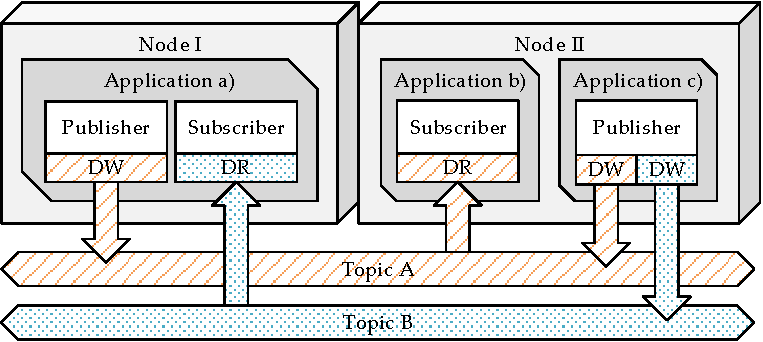
\includegraphics[width=0.8\textwidth]{figures/dds.pdf}
  \caption[An example of a distributed application connected via DDS]{An example of a distributed application connected via DDS}\label{fig:dds}
\end{figure}

\paragraph{Topics.}
\emph{Topics} form the basis on which peers communicate in the publish-subscribe paradigm. When a Publisher offers a certain kind of data, it does so by means of a Topic. When a data sample should be written, the Publisher pushes that data sample to a Topic appropriate for that sort of data. Conversely, when a Subscriber is interested in receiving data of a certain kind, then it subscribes to a Topic associated with that data. A Topic is uniquely defined by an identifier (name), a data type, and a set of QoS policies (see below). The data type represents the message format for data samples published on that Topic. For example, a suitable data type for a Topic concerned with temperature data would be a \texttt{struct} containing a single \texttt{float} value representing a temperature reading.
In \Cref{fig:dds} two Topics are depicted (Topic A and Topic B), each with a number of associated Data Writers and Data Readers (see below).

\paragraph{Publishers and Data Writers.}
\emph{Publishers} are entities that provide information in the publish-subscribe communication paradigm. Publishers are not bound to a single Topic. Instead, they contain one or more \emph{Data Writers}, each dedicated to a single Topic, who perform the actual data submission. Thus, Publishers may be seen as containers for a number of (unrelated) Data Writers. This concept is emphasized in \Cref{fig:dds} where a Publisher in Application c) controls two independent Data Writers that both write to different Topics.

\paragraph{Subscribers and Data Readers.}
\emph{Subscribers} are the exact compliment to Publishers in that they seek to receive data from Publishers. Analogous to Publishers, Subscribers are a way to group together sets of \emph{Data Readers}. Data Readers are entities whose purpose it is to receive data samples from their respective Topic. Through its API, DDS allows Data Writers to receive data in three ways: either by waiting for data samples (blocking the main thread), by pro-actively polling for new data samples, or by specifying asynchronous callbacks which are invoked whenever a data sample arrives.

\paragraph{Domains and Domain Participants.}
\emph{Domains} are the DDS way of grouping together sets of coherent \emph{Domain Participants} and to separate those sets from each other. Speaking in terms of distributed systems, Domains are a mechanism to manage group memberships of nodes \cite{tanenbaum2017distributed}. Domain Participants are entities that belong to a particular Domain. Each Publisher, Subscriber and Topic is derived from one Domain Participant and is therefore dedicated to exactly that Domain. As a consequence, participants of different Domains are entirely separated from each other and there is no way for them to interface with each other. Depicted in \Cref{fig:dds} is only one Domain. However, there could just as well be other Domains.
\pagebreak
\subsection{Quality of Service}
One of DDS's salient features is its intrinsic support for Quality of Service (QoS), which is realized by so-called ``QoS policies''. QoS policies specify attributes that can be used to control each component's behavior and quality properties. They make specifying a component's behavior a matter of \emph{configuration}, rather than \emph{implementation}. For example, consider a Data Writer which writes data to a Topic at a high rate. A Data Reader may be interested in that data but not at such a high rate, \eg\ because it runs on an embedded device powered by a battery and therefore needs to manage power consumption carefully. The Data Reader may now apply a \tbf , which instructs DDS to block all samples that exceed a specified frequency threshold. This way, the rate of incoming messages can be controlled via configuration. This is beneficial for the programmer as they do not need to accommodate for this at code level, but let the middleware take care of it.

QoS policies can be set for each Topic, Publisher, Subscriber, Data Writer and Data Reader individually.
In \Cref{tab:qos}, an excerpt of the available QoS policies is given. For the exhaustive list of all available QoS policies refer to the official standard \cite{dds-1.4-standard}.

Another example of a QoS policy is the \deadline\ policy. It specifies the minimum sampling frequency of a Data Writer. If the deadline period of a hypothetical Data Writer is set to, e.g., 100 ms, then this Data Writer is obligated to send a data sample at least every 100 ms. If it fails to send samples at this rate, the Data Writer and all the respective Topic's readers will be notified about that circumstance and are free to act accordingly.

In addition to specifying quality attributes, QoS policies may also serve as ``service contracts'' between interacting DDS components. These contracts specify non-functional requirements that the involved components must fulfill to be able to communicate with each other. For example, a Data Writer's \reliability\ policy may have been set to the \texttt{BEST\_EFFORT} level, thereby allowing the writer to drop samples. A Data Reader, on the other hand, may require the writer's policy to be set to \texttt{RELIABLE}, which prohibits the dropping of samples. Since the writer does not fulfill the reader's QoS requirements, the two components are considered incompatible, and thus, they cannot interact with each other.

Despite their name, QoS policies do not only concern \emph{quality} attributes per se. They can also be used to specify the priority of data samples, their lifespan, \ie , how long they are valid, or how many data samples of a certain type are kept in local memory.


\begin{table}[H]
  \caption[An excerpt of DDS QoS policies]{An excerpt of QoS policies}\label{tab:qos}
  \centering
  \begin{tabular}{p{0.25\textwidth} p{0.2\textwidth}  p{0.45\textwidth}}
    \toprule
      \textbf{Name} & \textbf{Legal values} & \textbf{Description} \\
    \midrule
    	\reliability  & \texttt{RELIABLE}, \texttt{BEST\_EFFORT} & Indicates whether a Data Writer may drop samples or whether a Data Reader approves of Data Writers that drop samples.\\
    	\tbf  & An integer value denoting time & Specifies a Data Reader's desired data reception rate. Superfluous samples will be discarded.\\
    	\liveliness  & An integer value denoting time & Defines the rules to determine whether a particular entity is ``alive'', \eg\ by emitting heart beats. \\
    	\deadline  & An integer value denoting time & Establishes a contract between Data Writer and Data Reader to determine the acceptable data rate. \\
    	\ownership  & \texttt{SHARED}, \texttt{EXCLUSIVE} & Specifies whether multiple Data Writers may write to a given Topic simultaneously or just the one with the highest \ostrength\  value.\\
    	\ostrength  & An integer value denoting relative priority & Determines a Data Writer's priority in cases where its Topic's \ownership\ is set to \texttt{EXCLUSIVE}. \\
    \bottomrule
  \end{tabular}
\end{table}
%
%
%
%
%
%
%
%
%
%
%
%
\pagebreak
\subsection{Redundancy and Automatic Failover} \label{sec:failover}
DDS has ways to ensure reliable communication---even over unreliable transmission channels. Part of reliability is failure transparency, \ie , the ability to quickly substitute failed components by backup components. The substitution process involves two steps: first, the failure needs to be detected. Second, a backup component needs to be instructed to take over. By means of the three QoS policies \ownership , \ostrength\ and \liveliness\ (\cf \Cref{tab:qos}), DDS may realize this process.

As the first step, a mechanism needs to determine whether a component has failed. In most cases, it is not possible for a failing component to properly shut down and ``sign off'', \ie , to notify the rest of the system that it will become unavailable. For this reason, the failure needs to be automatically registered. The \liveliness\ policy can be used to achieve this. \liveliness\ is the mechanism that determines whether a component is responsive (``alive''), or unresponsive (``dead''). The policy's value can be set to number indicating the maximum time interval between each liveliness signal. If a component fails to show a vital sign during that period, it is considered dead by the rest of the system. Passive components, \ie\ those which do not actively emit data, can be instructed to automatically send liveliness signals, or heartbeats, in certain intervals.

After a component has been declared dead it is up to the middleware to elect a substitute component. This is done through the \ownership\ and \ostrength\ QoS policies. By assigning a topic the \ownership\ value ``\qos{exclusive}'' one can specify that only a single data writer may write to that topic at any given time. Which data writer is given that prerogative is determined by the data writer's \ostrength\ value. The data writer that possesses the higher value is eligible to write to the topic. In the failover scenario, both, the primary data writer and the backup writer are assigned to the same topic, and both are configured to have exclusive \ownership\ rights. The former one has a higher \ostrength\ than the latter one. Based on both writer's \ostrength\ values, it is decided which one has precedence over the other.
%
%
%
%
%
%
%
%
%
%
%
%
%\subsection{Separation of User Data}
%The presented approach relies on a single cloud infrastructure, while at the same time, a vast number of customers need to be served. This poses a challenge concerning the separation of data. Confidentiality and privacy of user-specific application data must be preserved. Similarly, the result of a computation commissioned by a specific vehicle must be returned to exactly that vehicle, and no one else.

%Gladly, DDS offers a solution to this. In DDS, topics are not restricted to a single domain, \ie , they may be reused in multiple domains. If, \eg , a publisher belongs to \texttt{Domain $\alpha$} and publishes data on \texttt{Topic A}. Then, a data reader that reads from \texttt{Topic A} but belongs to \texttt{Domain $\beta$} may not read the data. Therefore, through domains, the same application may be reused several times on the same network, while keeping topic data separate. This principle is taken advantage of in the presented approach: domains are used to separate user data, such that for each user there is one user-specific domain. Thus, there is no way that data from one vehicle may interfere with data from another vehicle.

%\subsection{DDS for Automotive Systems}
%Automotive software systems have previously relied---and, to some degree, will continue to do so---on low-level, low-bandwidth transport protocols such as CAN, LIN, etc. For the longest time, networks stacks based on those protocols were sufficient to meet the basic requirements of delivering vehicular sensor data. However, driven by the emergence of innovative functions, the demands for vehicle intrinsic networks are skyrocketing. In particular, more and more sensor data from increasingly bandwidth-hungry sensors, such as cameras and lidars is feeding into advanced systems such as ADAS.
%At the same time, these functions require computational capabilities that go way beyond of what is possible with the microcontrollers typically used in traditional ECUs. High-performance computer systems based on high-level operating systems, supported by bandwidth-friendly networking protocols are needed to meet the new requirements.
%A new generation of low-level network protocols found their way into the vehicle. Notable mentions are FlexRay, and TSN. A question that remains is whether DDS is a suitable choice for the use within vehicles, and whether DDS may be used efficiently on top of these lower level protocols. \citeauthor*{bouhouch2013dds} have shown \cite{bouhouch2013dds} that DDS is indeed a suitable middleware to be used in vehicular networks.

%DDS allows to configure how much of a system's resources an DDS-enabled application may use. Consequently, it is the middleware's responsibility to allocate resources as needed while still staying within the specified boundaries. At the same time, priorities aligning with the application's QoS settings need to be considered. DDS takes this burden off the programmer's shoulders.
%\todo[inline]{TODO}


%
%
%
%
%
%
%
%
%
%
%
%
%
%
%
%
%
%
%
%


%
%
%
%
%
%
%
%
%
%

\section{\docker\ for Containerization}
In this thesis' approach, services and their dependencies shall be encapsulated in their own, self-contained execution environments that may be deployed inside the vehicle and also in the cloud. Containerization is a promising technology to achieve this. For the exemplary implementation, \docker\ is used as it provides an easy-to-use interface and is available for x86, as well as for ARM-based platforms.

\docker\ is a holistic containerization platform which includes everything needed to build, run, deploy, and distribute containers. The \docker\ application is structured in a client-server model (\cf \Cref{fig:docker-arch}). The server is a daemon process running at all times on the host machine. Its primary purpose is to manage containers, images, networks and data volumes, and to provide the means to  build images and run containers. The \docker\ server exposes a RESTful HTTP API by which it can be controlled. The client side of the \docker\ application is a command line interface (CLI) which acts as a user friendly façade for the server's API.\footnote{\url{docs.docker.com/engine/docker-overview}}

\begin{figure}[htpb]
  \centering
  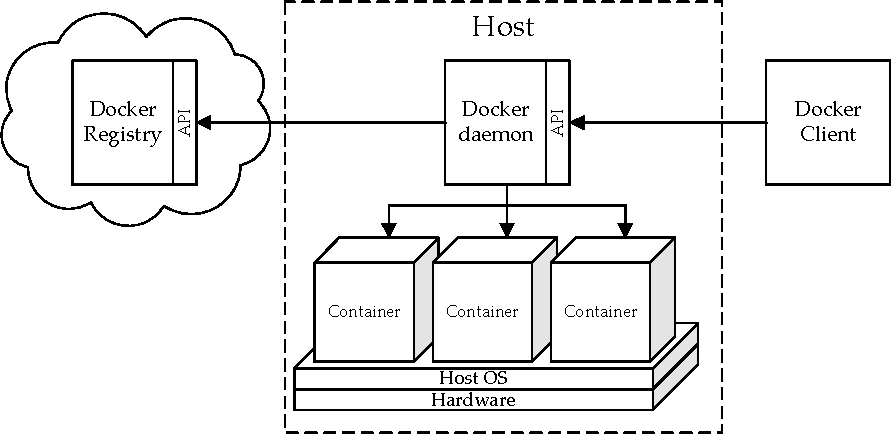
\includegraphics[width=0.9\textwidth]{figures/docker-arch.pdf}
  \caption[\docker\ architecture]{\docker\ architecture}\label{fig:docker-arch}
\end{figure}

\subsection{\docker\ Components}
\paragraph{\docker\ Images.}
Images are a central component of \docker . They may be seen as the ``blueprint'' on the basis of which containers are built and define exactly which files and directories are contained in a container once it comes to life. Effectively, every container is an instantiation of an image of a certain type, in the same way an object is an instantiation of a class in an object-oriented programming language. While the concept of images is very common among containerization and virtualization tools, \docker\ follows a rather unconventional approach.
In \docker , images are made up of series of read-only file system layers stacked on top of each other. Each layer may add files and directories to its respective underlying layer. If a layer tries to modify a file from an underlying layer it creates a copy of that file and adds it to its own layer. The modification is then performed on the copy instead of the original. This principle called ``Copy on Write'' (CoW) ensures that layers cannot be modified which makes it possible to share individual layers with other images stored on the host. An example of this is later described in \Cref{sec:containerized-services}. By treating images as a collection of individual, sharable pieces instead of atomic units, massive storage space savings can be achieved. Another benefit of this is that whenever a container is started, only a thin writable layer needs to be added on top of an image, and the underlying layers do not need to be copied. That way, start-up times of containers are kept extremely low.\footnote{\url{docs.docker.com/storage/storagedriver}} \todo{how low? quellen} Virtual Machines, in contrast, would first need to boot into an operating system prior to operation.
\todo[inline]{Image of layered image?}

\paragraph{Dockerfiles.}
\docker\ images are defined in so-called Dockerfiles.\footnote{\url{docs.docker.com/engine/reference/builder}} Dockerfiles are made up of series of instructions that tell \docker\ how to build a certain image. Each instruction adds another file system layer to the image.
\begin{lstlisting}[caption=An examplary Dockerfile, label=lst:dockerfile, numbers=left, numberstyle=\tiny]
FROM debian
COPY . /application
RUN cd /application && make
ENTRYPOINT /application/run.sh
\end{lstlisting}
An example of a Dockerfile is depicted in \Cref{lst:dockerfile}. The first line of this Dockerfile defines the base image on top of which this particular image shall be built. In this case, an image called ``debian'' was chosen. As the name suggests, that base image contains a basic installation of the Linux distribution Debian.\footnote{\url{www.debian.org}} Next, the line \ \mbox{\texttt{COPY . /application}} \ instructs \docker\ to copy the contents of the current (host) directory to the container's \ \mbox{\texttt{/application}} \ directory. Due to \docker 's CoW approach, the changes in the file system are added in the form of a layer---the underlying layers are not affected. The \ \texttt{RUN} \ instruction in the following line causes \docker\ to run the subsequent commands within the container. In this case, the newly added application directory is entered and the command \ \texttt{make} \ is executed, effectively compiling the application. Again, the resulting changes to the file system are encapsulated within another layer. In practice, the now topmost layer would contain all files produced by \ \texttt{make}. Finally, the \ \mbox{\texttt{ENTRYPOINT}} \ instruction defines the action to be performed once the container is started. In this case, the shell script \ \texttt{run.sh} \ would be executed within the container. This command, too, would add a layer to the image, albeit an empty one. By defining images as sequences of instructions, reproducibility is guaranteed.
By running the command \ \mbox{\texttt{docker build -t IMAGENAME .}} \ in the directory of the Dockerfile, an image based on that Dockerfile would be built. Using the command \ \mbox{\texttt{docker run IMAGENAME}}, a new container of that image type would be launched.

\paragraph{\docker\ Registries.}
\docker\ images may be stored in \docker\ Registries,\footnote{\url{docs.docker.com/registry}} where they can be browsed, managed, and distributed. The command \ \mbox{\texttt{docker push IMAGENAME[:TAG]}} \ causes the image with the name \ \mbox{\texttt{IMAGENAME}} \ to be uploaded to a registry. Analogously, to download an image from a registry to the local computer, one would have to run the command \ \mbox{\texttt{docker pull IMAGENAME[:TAG]}}. \docker\ registries are implemented as a server software which exposes an HTTP API (\cf \Cref{fig:docker-arch}). The registry server is open source\footnote{\url{www.github.com/docker/distribution}} and may be deployed on any server that supports it. The \docker\ company itself hosts one of such registries, Docker Hub,\footnote{\url{hub.docker.com}} which is provided as a publicly available  and free-to-use service.

\subsection{Multi Platform Compatibility} \label{sec:multiplat}
The primary purpose of containerization is to provide portable execution environments that allow software to run on a broad range of computing systems. A limitation of containers is that they only provide portability across \emph{operating systems}, and not \emph{hardware platforms}. In other words, containers do not provide binary compatibility. The reason for this is that containerized applications run directly on the kernel of the host system, and do not build on top of a virtualization layer as classic VMs do. As a result, a containerized binary built for an x86-based processor will not run on an ARM system, and vice versa. This is problematic especially in the context of embedded systems which often rely on particular hardware architectures that favor energy efficiency over performance. Computing nodes in a data centers, on the other hand, are typically based on architectures aimed at providing a maximum level of performance. As the presented approach intends containers to be deployed on both, vehicular on-board systems and in the cloud, this poses a challenge. Two approaches exist to tackle this problem.

\subsubsection{Universal, QEMU-enabled Images}
The first approach relies on a thin platform compatibility layer that is put into the base of each container. This approach was popularized by resin.io, a company that specializes in containerization for IoT devices. On their Docker Hub page\footnote{\url{hub.docker.com/u/resin}} they provide \docker\ images which have the QEMU\footnote{\url{www.qemu.org}} machine emulator built in. Facilitated by QEMU's user emulation mode, binaries built for a given processor architecture may be executed on otherwise incompatible processors. QEMU achieves this by translating any guest system calls into host system calls. The previously mentioned images are built in a way that allows any arbitrary binary executed within such container to be run in the context of QEMU. Thus, the container may run on a multitude of hardware platforms.
This approach simplifies the software build process tremendously as only one universal container per service needs to be built. This container can then be reused for all platforms.

\subsubsection{Manifest Lookup}
The QEMU approach has a significant drawback: multicast is not well supported by QEMU, which is why the idea was discarded.
Thus, another approach was leveraged to solve the multi-platform compatibility issue. This approach builds on Continuous Integration (CI) in accord with Docker Hub, and in particular, Docker Hub's \emph{image manifest} feature. The concept of image manifests builds on the following premise: by default, a \docker\ image name corresponds to exactly \emph{one} image. Thus, whenever an image with a given name is requested from the \docker\ registry, only that specific image is returned to the requester. Image manifests extend registries by the option to define \emph{multiple} images per image name. That way, several containers, each specifically built for a given platform, may be deployed under the same name. Depending on the requesting node's hardware architecture, a different image may be returned. \Cref{fig:manifest-pull} depicts an example for this. In the example, an x86-based machine requests the \ \mbox{\texttt{some/image:v1.0}} \ image from the registry. What is then returned from the registry is an image specifically made for x86 architectures. On the other hand, an ARM-based machine which requests the very same image, \ \mbox{\texttt{some/image:v1.0}}, receives an entirely different image as a response. This kind of behavior is achieved through an image lookup in the manifest file which is performed behind the scenes.

\begin{figure}[htpb]
  \centering
  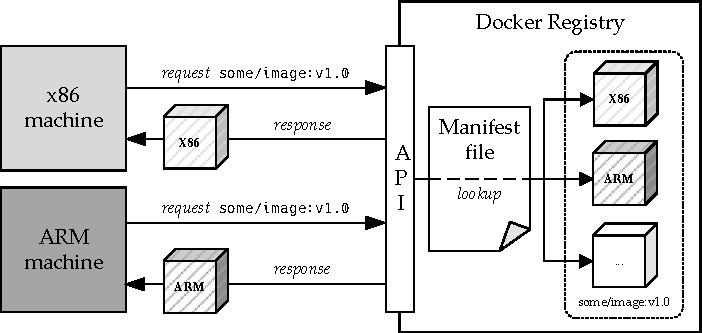
\includegraphics[width=0.8\textwidth]{figures/manifest-pull}
  \caption[Pulling \docker\ images via manifest file]{Two nodes request the same image name but receive different images which are specifically built for their respective processor architecture. Which node requires which image is determined by a look-up in the manifest file.}\label{fig:manifest-pull}
\end{figure}

A disadvantage of this approach (compared to the QEMU one) is that multiple versions of the same container need to be built every time a service receives a software update. To cope with this hindrance, a minimal CI pipeline was leveraged. Consider \Cref{fig:manifest-push} in which the employed service deployment process is depicted. The build process is initiated whenever a code change is pushed to the remote git repository. Once a push is registered, the CI Platform (Travis CI\footnote{\url{www.travis-ci.org}} was used) pulls the latest version from the git repository and executes a build script. The build script compiles several version of the service for each target platform, embeds the binaries in images and pushes those images to the \docker\ registry (Docker Hub). Thus, several images, each tailored to a different platform, may be built and deployed in one go.

\begin{figure}[htpb]
  \centering
  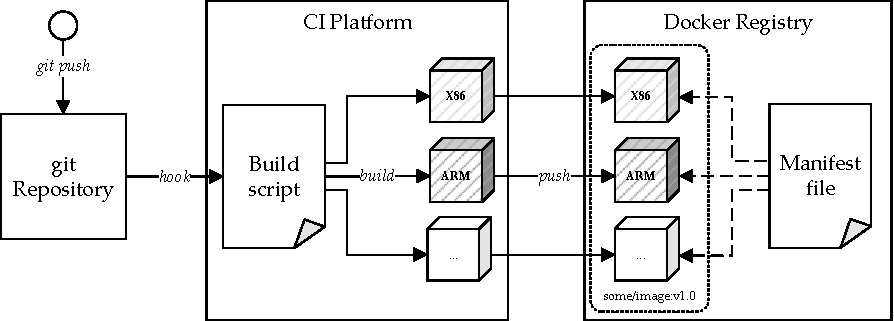
\includegraphics[width=\textwidth]{figures/manifest-push}
  \caption[Pushing \docker\ images via CI]{A git push to a service's git repository triggers the build process in the CI platform: the code is compiled for several platforms and the resulting images are pushed to the \docker\ registry.}\label{fig:manifest-push}
\end{figure}

%
%
%
%
%
%
%
%
%
%
%
\subsection{Containerized Services} \label{sec:containerized-services}
In the envisaged system, each service is packed into its own container with all its dependencies. That way, services may run wherever they are placed, and thus, a great deal of portability is achieved.

\Cref{fig:service-containers} shows an example of three containerized services running on two different machines, \experim{Host I} and \experim{Host II}. On the former, two instances of \experim{Service A}, and one instance of \experim{Service B} are placed. On the second host only one service instance is deployed, namely one of type \experim{Service C}. All services are packaged in their own, separate container. The containers are made up of three stacked images---the bottom two are common to all services. The bottommost image (``\emph{base image}'') contains the file system layers of a minimal operating system. In this thesis, the Linux distribution Debian was used. The base image only contains a limited selection of Linux tools, such as \ \texttt{ls}, \texttt{cat}, \texttt{ps} \ etc. The purpose of a base image is to lay a solid foundation that enables users to work comfortably within the container. In the case of Debian, the \emph{aptitude} package manager is additionally included which enables users to easily install further tools.

\begin{figure}[htpb]
  \centering
  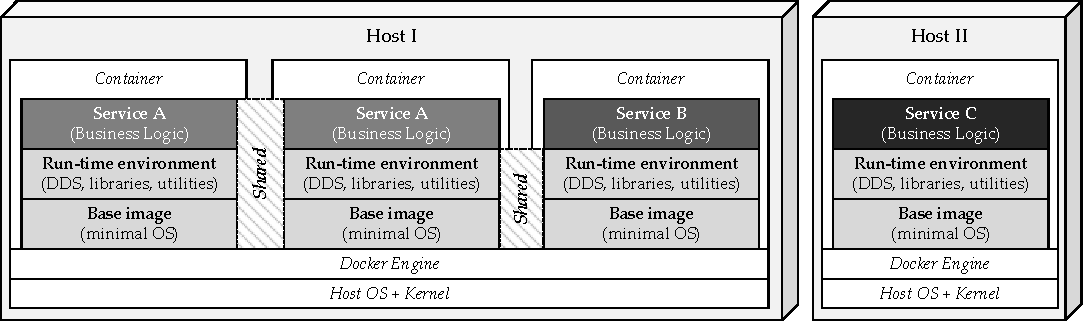
\includegraphics[width=\textwidth]{figures/docker-sharing}
  \caption[An example of containerized services]{An example of four containerized service instances, some sharing common logic to save disk space and facilitate fast updates}\label{fig:service-containers}
\end{figure}

Next, an \emph{intermediate image} is built on top of the base image. The intermediate image adds further layers containing the services' run-time environment, and in particular, the shared libraries of OpenDDS. This image could optionally contain additional libraries and tools that are common to all services. For the purpose of demonstration, however, DDS on its own is sufficient. The base image and the intermediate image lay the foundation of all services. Any image built on top of these could run any DDS-enabled application. Facilitated by \docker 's layered approach to images, the bottom two images can be shared among all services deployed on a host. In the example, the base image and the intermediate image both only need to be stored once on \experim{Host I}, which saves tremendous amounts of disk space.

At the top, finally, sit the \emph{service images}. In these images contained is the actual service logic, and more precisely, the service's binary and configuration files. The service images are unique to each service, and are not shared, except when the same service is instantiated multiple times on the same machine (\cf \experim{Service A} in \Cref{fig:service-containers}).



\section{Container Networking with \wnet}
\wnet\ is an open source project\footnote{\url{www.github.com/weaveworks/weave}} which is developed by a global team, mostly employed by the London-based software company \emph{Weaveworks}\footnote{\url{www.weave.works}}. The purpose of \wnet\ is to provide advanced overlay networking capabilities for \docker\ containers. As such, is designed to make up for the shortcomings of \docker 's built-in overlay networks, and more specifically, their lack of encryption and multicast support. By means of \weave\ overlay networks, dispersed containers deployed on physically isolated hosts around the world, may communicate as if they were connected via LAN. From a containerized applications' viewpoint, it does not matter whether its peers are located on the same host or within a data center on the other side of the world. 

\paragraph{}

\wnet\ is implemented as client software which is installed on each machine that partakes in the overlay. The software can be started using a single command, and in the following, all containers launched on that host will automatically connected to the overlay network. This is achieved by means of a \emph{\docker\ API proxy}. The proxy sits between \docker 's command-line client and the \docker\ daemon and intercepts all communication between the two. When the \docker\ engine is instructed to start a container, the proxy takes all precautions needed to enable overlay networking for that container. Once the connection is established, all container traffic is routed through three dedicated network channels: one TCP connection to exchange meta data about the network, and two UDP channels for duplex data exchange.

\begin{figure}[htpb]
  \centering
  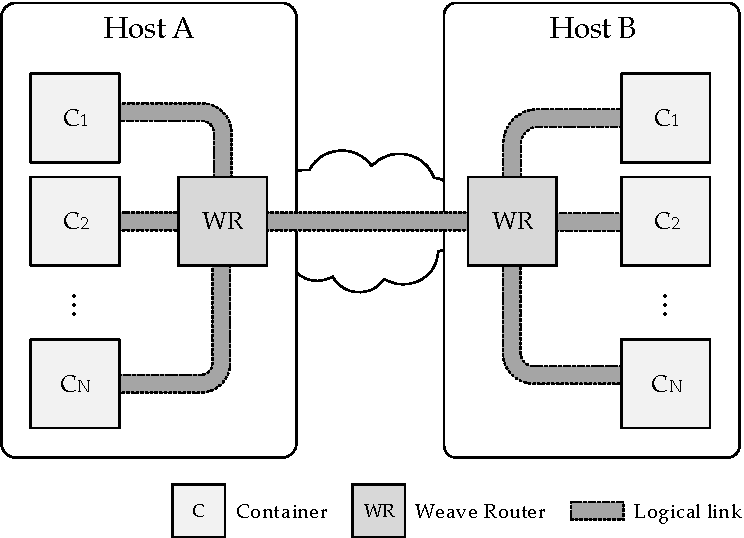
\includegraphics[width=0.7\textwidth]{figures/weave.pdf}
  \caption[An example of containers connected via \wnet\ overlay network]{A number of dispersed containers connected by a \wnet\ overlay network}\label{fig:weavescheme} 
\end{figure}

When the \weave\ software is started, a central component of \wnet , the \emph{\weave\ router} is launched (\cf\ \autoref{fig:weavescheme}). Similar to a hardware router, the \weave\ router is responsible for the forwarding and routing of data packets to their appropriate receivers. \weave\ routers can be seen as gateways through which all containers participating in a \weave\ network are connected. To facilitate routing on the data plane, a custom UDP encapsulation protocol, called \emph{sleeve}, was devised. A \weave\ router in itself is an containerized application running at all times, in the same way a daemon would. There is one of such router containers running on every host in a \weave -enabled infrastructure.

\todo[inline]{ÜBERARBEITEN}

The \weave\ router is a user space process. As such, a context switch is needed every time it is tasked to process a packet. This comes with a substantial performance overhead. Hence, as a faster alternative, the so-called \emph{fast datapath} mode was added. In this mode, packets are processed by the Linux kernel instead of by the \weave\ router. This way, the context switch into user space is omitted. \wnet\ leverages the Linux kernel's \emph{Open vSwitch datapath} module \cite{pfaff2015design} to achieve this behavior. Open vSwitch can be used to create a virtual, software-based network switch. That way, the kernel can be instructed to process packets in a certain way. For instance, the kernel can be commanded to add a VXLAN header to each packet, thereby achieving the same result as the \weave\ router, but faster. However, fast datapath mode can only be used when the underlying infrastructure allows it. The Internet is a particular example of a network where fast datapath communication is hard to achieve.


\subsection{Topology Management} 
\weave 's topology management is self-governing and self-healing. Peers continually exchange topology information and monitor the state of the network. Whenever peers lose connectivity, they continuously try to re-establish the connection until it is restored. All participating peers know the topology of the entire network. For this, \wnet\ employs a sophisticated discovery and topology management mechanism by which changes in the network topology are rapidly propagated within the network. The topology management protocol is based on a spanning-tree broadcast mechanism known from hardware switches. To further ensure that all peers have an up-to-date neighbor list at all times, \wnet\ additionally employs a custom neighbor gossiping protocol by which each peer sends update messages to a random subset of their neighbors. Updates of the network's topology are performed periodically as well as when certain events occur, such as when a node joins or leaves the network.

In order to add a new host to the overlay, the \weave\ software needs to be started on that host, referencing at least one other host in the network by its IP address. The information that a new host was added is then propagated to the other hosts in the overlay. After a short period, all hosts know that the new host was added and that a path to that host exists.

\subsection{Encryption} 
As mentioned earlier, a salient feature of \wnet\ is the ability to encrypt all traffic within the overlay network\footnote{Encryption applies end-to-end between \weave\ routers}. This is especially important for networks that span over insecure underlays, such as the Internet. To set up encryption, a shared secret (password) needs to be provided when the \weave\ router is launched. The shared secret must therefore be present on all participating hosts. From the password, salted, ephemeral session keys are generated which are then used to encrypt the network packets' payload. For each connection between any two peers, one unique session key exists.

The way encryption is applied differs depending on the forwarding mode used (sleeve or fast datapath). In fast datapath mode, a IPsec-based protocol is used, whereby each packet is wrapped in an encapsulated security payload (ESP). Because each packet in this mode is processed by the Linux kernel, encryption is applied by means of the standard Linux Kernel Crypto API which is thoroughly tested, and generally considered secure. For sleeve mode, a custom encryption algorithm based on TLS\footnote{``Transport Layer Security''} is used. As with fast datapath encryption, sleeve mode encryption utilizes shared, ephemeral session keys for each connection.

\begin{figure}[htpb]
  \centering
  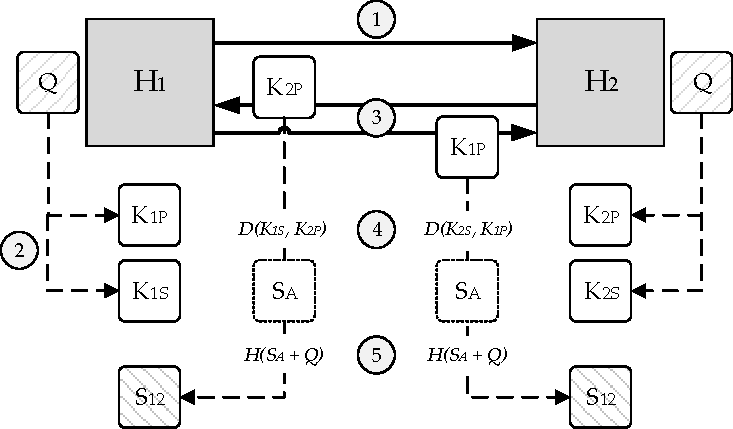
\includegraphics[width=0.6\textwidth]{figures/weave-encryption.pdf}
  \caption[\weave 's key exchange protocol]{\wnet 's key exchange protocol in sleeve mode}\label{fig:weaveencryption}
\end{figure} 
\autoref{fig:weaveencryption} depicts how these session keys are generated. In the image, two hosts ($H_1$, $H_2$) are to establish an encrypted connection. First, $H_1$ initiates the key exchange by sending a handshake message to $H_2$ \circled{1}. Then, both hosts generate their own, individual key pairs so that each host has a public key and a private key \circled{2}. The key pair for $H_1$ is $(K_{1P}, K_{1S})$ and the key pair for $H_2$ is $(K_{2P}, K_{2S})$. Once that is done, both hosts exchange their respective public keys, $K_{1P}$, and $K_{2P}$ \circled{3}. Using the peer's public key and their own private key, both hosts derive an auxiliary shared key, $S_A$, by means of Diffie--Hellman key exchange \cite{bresson2001provably}: $D(K_{1S},K_{2P})$ \circled{4}. Finally, the actual shared key can be generated. For this, both hosts append the password ($P$) to $S_A$ to provide authenticity. In order to bring the key to the desired length of 256 bit, the compounded key is additionally hashed via SHA256: $H(S_A, P)$ \circled{5}. The end result of this procedure is the final shared key, $S_{12}$, which is then used to encrypt the traffic between the two hosts.
%
%
%
%
%
%
%
%
%
%
%
%
%
%
%
%
%
%
%
%








